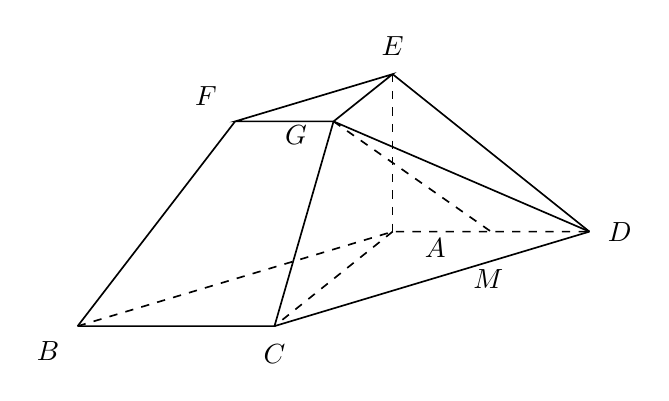
\begin{tikzpicture}[x=1cm,y=1cm,font=\normalsize,line width=.6pt]
\coordinate (B) at (0,0);
\coordinate (C) at (2.5,0);
\coordinate (A) at (4.0000000000,1.2000000000);
\coordinate (D) at (6.5000000000,1.2000000000);
\coordinate (M) at (5.2500000000,1.2000000000);
\coordinate (E) at (4.0000000000,3.2000000000);
\coordinate (F) at (2.0000000000,2.6000000000);
\coordinate (G) at (3.2500000000,2.6000000000);
% bottom face
\draw[solid] (B) -- (C) -- (D);
\draw[dashed] (B) -- (A) -- (D);
\draw[dashed] (A) -- (C);
% top small triangle / quadrilateral
\draw[solid] (E) -- (F) -- (G) -- cycle;
\draw[solid] (F) -- (B);
\draw[solid] (E) -- (D);
\draw[solid] (G) -- (C);
\draw[solid] (G) -- (D);
% vertical / hidden
\draw[dashed] (E) -- (A);
\draw[dashed] (G) -- (M);
% labels offset outward
\node[below left,xshift=-3pt,yshift=-2pt] at (B) {$B$};
\node[below,xshift=0pt,yshift=-3pt] at (C) {$C$};
\node[right,xshift=8pt,yshift=-6pt] at (A) {$A$};
\node[right,xshift=3pt] at (D) {$D$};
\node[above,xshift=0pt,yshift=3pt] at (E) {$E$};
\node[above left,xshift=-3pt,yshift=2pt] at (F) {$F$};
\node[left,xshift=-6pt,yshift=-5pt] at (G) {$G$};
\node[below=3pt,xshift=-1pt,yshift=-7pt] at (M) {$M$};
\end{tikzpicture}
